\documentclass[12pt]{article}

\usepackage[top = 1in, bottom = 1in, left = 0.75in, right = 0.75in]{geometry}
\usepackage{amsmath, amssymb, amsthm}
\usepackage{graphicx}
\usepackage{float}
\usepackage{tikz}
\usetikzlibrary{shapes.geometric, arrows}

\tikzstyle{arrow} = [thick,->,>=stealth]
\tikzstyle{process} = [circle, minimum width=1.5cm, minimum height=1.5cm, text centered, draw=black]


\theoremstyle{definition}
\newtheorem{question}{Question}
\newenvironment{answer}{
    \textbf{\textit{Answer:}} \qquad
}{\hfill $\blacksquare$ \\ 

\begin{center}
    \rule{0.8\linewidth}{1.5px} 
    \vspace*{1cm}   
\end{center}
%\pagebreak
}


% CUSTOM DEFINITIONS
\newcommand{\R}{\mathbb{R}}
\newcommand{\Z}{\mathbb{Z}}
\newcommand{\C}{\mathbb{C}}
\newcommand{\zcal}{\mathcal{Z}}
\newcommand{\inv}[1][1]{^{(- #1)}}


\title{Solution to Signal Processing Assignments 2}
\author{Subhrajyoty Roy (MB1911)}
\date{\today}

\begin{document}
\maketitle

\begin{center}
    \rule{0.8\textwidth}{1px} 
\end{center}
\vspace*{2em}

% DONE 
% Q1
\begin{question}
    Compute the convolution $y(n)$ of the signals
    $$
    x(n) = \begin{cases}
        \alpha^n & -3 \leq n \leq 5\\
        0 & \text{elsewhere}
    \end{cases} \qquad 
    h(n) = \begin{cases}
        1 & 0 \leq n \leq 4\\
        0 & \text{elsewhere}
    \end{cases}
    $$
\end{question}

\begin{answer}
    In this case, we shall use \textbf{Overlap and Add Method} to compute the discrete convolution $y(n) = x(n) \ast h(n)$.

    \begin{table}[H]
        \centering
        \begin{tabular}{r|ccccc}
             & $\stackrel{\downarrow}{1}$ & 1 & 1 & 1 & 1\\
             \hline
            $\alpha^{(-3)}$ & $\alpha^{(-3)}$ & $\alpha^{(-3)}$ & $\alpha^{(-3)}$ & $\alpha^{(-3)}$ & $\alpha^{(-3)}$ \\
            $\alpha^{(-2)}$ & $\alpha^{(-2)}$ & $\alpha^{(-2)}$ & $\alpha^{(-2)}$ & $\alpha^{(-2)}$ & $\alpha^{(-2)}$ \\
            $\alpha^{(-1)}$ & $\alpha^{(-1)}$ & $\alpha^{(-1)}$ & $\alpha^{(-1)}$ & $\alpha^{(-1)}$ & $\alpha^{(-1)}$ \\
            $\rightarrow 1$ & 1 & 1 & 1 & 1 & 1\\
            $\alpha$ & $\alpha$ & $\alpha$ & $\alpha$ & $\alpha$ & $\alpha$\\
            $\alpha^2$ & $\alpha^2$ & $\alpha^2$ & $\alpha^2$ & $\alpha^2$ & $\alpha^2$\\
            $\alpha^3$ & $\alpha^3$ & $\alpha^3$ & $\alpha^3$ & $\alpha^3$ & $\alpha^3$\\
            $\alpha^4$ & $\alpha^4$ & $\alpha^4$ & $\alpha^4$ & $\alpha^4$ & $\alpha^4$\\
            $\alpha^5$ & $\alpha^5$ & $\alpha^5$ & $\alpha^5$ & $\alpha^5$ & $\alpha^5$\\
        \end{tabular}
    \end{table}

    Thus, we have the output sequence given as 


    \begingroup
    \allowdisplaybreaks
    \begin{align*}
        y(-3) = \alpha^{(-3)}, 
        & \qquad y(-2) = \alpha^{(-2)} (1 + \alpha^{(-1)})\\
        y(-1) = \alpha^{(-3)} \dfrac{(1 - \alpha^3)}{(1 - \alpha)}, & \qquad 
        y(0) = \alpha^{(-3)} \dfrac{(1 - \alpha^4)}{(1 - \alpha)},\\
        y(1) = \alpha^{(-3)} \dfrac{(1 - \alpha^5)}{(1 - \alpha)}, & \qquad
        y(2) = \alpha^{(-2)} \dfrac{(1 - \alpha^5)}{(1 - \alpha)} \\
        y(3) = \alpha^{(-1)} \dfrac{(1 - \alpha^5)}{(1 - \alpha)}, & \qquad
        y(4) = \dfrac{(1 - \alpha^5)}{(1 - \alpha)}, \\
        y(5) = \alpha \dfrac{(1 - \alpha^5)}{(1 - \alpha)}
        & \qquad
        y(6) = \alpha^2 \dfrac{(1 - \alpha^4)}{(1 - \alpha)},\\
        y(7) = \alpha^3 \dfrac{(1 - \alpha^3)}{(1 - \alpha)}, 
        & \qquad 
        y(8) = \alpha^4 (1 + \alpha), \qquad
        y(9) = \alpha^5
    \end{align*}
    \endgroup
\end{answer}


% DONE
% Q2
\begin{question}
    Determine the particular solution of the difference equation 
    $$
    y(n) = \dfrac{5}{6} y(n-1) - \dfrac{1}{6} y(n-2) + x(n)
    $$

    when the forcing function is $x(n) = 2^n u(n)$.
\end{question}

\begin{answer}
    Let, $Y(z)$ denote the $\zcal$-transform of $y(n)$ and $X(z)$ denote the $\zcal$-transform of $x(n)$. Then, we have

    \begin{equation*}
        X(z) = \sum_{n = 0}^{\infty} 2^n z^{(-n)} = \dfrac{1}{(1 - 2z\inv)}
    \end{equation*}
    
    Therefore, from the given difference equation and applying the time delay property of $\zcal$-transform, we obtain  

    \begin{align*}
        & Y(z) = \dfrac{5}{6} z\inv Y(z) - \dfrac{1}{6} z\inv[2] Y(z) + X(z)\\
        \Rightarrow \qquad & Y(z)\left(1 - \dfrac{5}{6}z\inv + \dfrac{1}{6}z\inv[2] \right) = \dfrac{1}{(1 - 2z\inv)} \\
        \Rightarrow \qquad & Y(z) \left( 1 - \dfrac{1}{2}z\inv\right) \left( 1 - \dfrac{1}{3}z\inv\right) = \dfrac{1}{\left( 1 - 2 z\inv \right)}\\
        \Rightarrow \qquad & Y(z) = \dfrac{1}{\left( 1 - \dfrac{1}{2}z\inv\right) \left( 1 - \dfrac{1}{3}z\inv\right)\left( 1 - 2 z\inv \right)} \\
        \Rightarrow \qquad & Y(z) =  \dfrac{A}{\left( 1 - \dfrac{1}{2}z\inv\right)} + \dfrac{B}{\left( 1 - \dfrac{1}{3}z\inv\right)} + \dfrac{C}{\left( 1 - 2z\inv\right)}
    \end{align*}

    where 

    \begin{align*}
        A & = \left. Y(z)\left( 1 - \dfrac{1}{2}z\inv\right) \right\vert_{z\inv = 2} =  (-1)\\
        B & = \left. Y(z)\left( 1 - \dfrac{1}{3}z\inv\right) \right\vert_{z\inv = 3} =  \frac{2}{5}\\
        C & = \left. Y(z)\left( 1 - 2z\inv\right) \right\vert_{z\inv = 1/2} = \frac{8}{5}
    \end{align*}

    Thus,

    $$
    Y(z) = -\dfrac{1}{\left( 1 - \dfrac{1}{2}z\inv\right)} + \dfrac{2}{5} \times \dfrac{1}{\left( 1 - \dfrac{1}{3}z\inv\right)} + \dfrac{8}{5} \times \dfrac{1}{\left( 1 - 2z\inv\right)}
    $$

    Note that since $\dfrac{1}{2} < 1$ and $\dfrac{1}{3} < 1$, the first two parts are causal, while the final term corresponds to an anti-causal system. Hence, inverting the above $\zcal$-transform would yield

    $$
    y(n) = \left[ -\left(\dfrac{1}{2}\right)^n + \dfrac{2}{5} \left(  \dfrac{1}{3}\right)^n \right] u(n) - \dfrac{8}{5} 2^n u(-n-1)
    $$
    
    which is the particular solution to the above difference equation.

\end{answer}

% Q3
\begin{question}
    Consider the signal $\gamma(n) = a^n u(n), 0 < a < 1$.
    \begin{enumerate}
        \item[(a)] Show that any sequence $x(n)$ can be decomposed as
        $$
        x(n) = \sum_{k = -\infty}^{\infty} c_k \gamma(n-k)
        $$ 
        and express $c_k$ in terms of $x(n)$.
        \item[(b)] Use the properties of linearity and time invariance to express the output $y(n) = \tau[x(n)]$ in terms of the input $x(n)$ and the signal $g(n) = \tau[\gamma(n)]$, where $\tau$ is an LTI system.
        \item[(c)] Express the impulse response $h(n) = \tau[\delta(n)]$ in terms of $g(n)$.  
    \end{enumerate} 
\end{question}

\begin{answer}
    \begin{enumerate}
        \item[(a)] Let us denote the sequence $c_k$ as $c(k)$, then
        
        $$
        \sum_{k = -\infty}^{\infty} c(k)\gamma(n-k) = c(n) \ast \gamma(n)
        $$

        where $\ast$ denotes the discrete convolution operator. Considering this, we first try to express the unit impulse response function $\delta(n)$ as the above convolution for some choice of $c(n)$'s. For that, we consider the following in the $\zcal$-domain

        \begin{align*}
            \zcal\{ \delta(n) \}
            = 1
            & = (1 - az\inv) \dfrac{1}{(1 - az\inv)}\\
            & = \zcal\{ \delta(n) - a \delta(n-1) \} \zcal\{ a^n u(n) \}\\
            & = \zcal\{ \delta(n) - a \delta(n-1) \} \zcal\{ \gamma(n) \}\\
            & = \zcal\{ b(n) \ast \gamma(n) \}, \\
            & \qquad \qquad \text{since, the discrete convolution becomes multiplication in } \zcal \text{ domain}
        \end{align*}

        where $b(n) = \delta(n) - a\delta(n-1)$. Thus, inverting the $\zcal$-transformation back to the time domain, we have 
        
        $$
        \delta(n) = b(n) \ast \gamma(n) = \sum_{k = -\infty}^{\infty} b(k) \gamma(n-k)
        $$

        Now, turning our attention to any sequence $x(n)$, we note that 

        \begin{align*}
            x(n)
            & = \sum_{k = -\infty}^{\infty} x(k) \delta(n-k)\\
            & = x(n) \ast \delta(n)\\
            & = x(n) \ast (b(n) \ast \gamma(n))\\
            & = (x(n) \ast b(n)) \ast \gamma(n) \qquad \text{by associativity of discrete convolution}\\
            & = c(n) \ast \gamma(n), \qquad \text{ where } c(n) = x(n) \ast b(n)
        \end{align*}

        In explicit terms,

        \begin{align*}
            c(n) 
            & = x(n) \ast (\delta(n) - a\delta(n-1))\\
            & = x(n) \ast \delta(n) - a x(n) \ast \delta(n-1)\\
            & = x(n) - ax(n-1)            
        \end{align*}

        Thus, once we expand the discrete convolution as infinite summation, we obtain

        $$
        x(n) = \sum_{k = -\infty}^\infty (x(k) - a x(k-1)) \gamma(n-k)
        $$

        Hence, any sequence $x(n)$ can be decomposed as
        
        $$
        x(n) = \sum_{k = -\infty}^\infty c_k \gamma(n-k)
        $$

        where $c_k = (x(k) - ax(k-1))$.

        \item[(b)] Let, $\tau$ be a linear and time invariant system. Hence,
        
        \begin{align*}
            \tau[x(n)]
            & = \tau\left[ \sum_{k = -\infty}^\infty c_k \gamma(n-k) \right]\\
            & = \sum_{k = -\infty}^\infty c_k \tau[\gamma(n-k)], \qquad \text{by linearity of }\tau\\
            & = \sum_{k = -\infty}^\infty c_k g(n-k), \qquad \text{by time invariance of } \tau\\
            & \qquad \qquad \text{ where } g(n) = \tau[\gamma(n)]\\
            & = \sum_{k = -\infty}^\infty (x(k) - ax(k-1)) g(n-k), \qquad \text{from part (a)}\\
        \end{align*}

        \item[(c)] Following part (b), the impulse response $h(n) = \tau[\delta(n)]$ can be expressed as,

        \begin{align*}
            h(n)
            & = \tau[\delta(n)]\\
            & = \sum_{k = -\infty}^\infty (\delta(k) - a\delta(k-1)) g(n-k)\\
            & = \sum_{k = -\infty}^\infty \delta(k) g(n-k) - a \sum_{k = -\infty}^\infty \delta(k-1)g(n-k)\\
            & = g(n) - a g(n-1)
        \end{align*}

        since in the first summation, $\delta(k) \neq 0$ if and only if $k = 0$, and thus only the term corresponding $g(n)$ will be remain, while in the second summation $\delta(k-1) \neq 0$ if and only if $k = 1$, thus only $g(n-1)$ remained.
    \end{enumerate}
\end{answer}


% DONE
% Q4
\begin{question}
    Determine the impulse response of the following causal system 
    $$
    y(n) - 3 y(n-1) - 4y(n-2) = x(n) + 2x(n-1)
    $$
\end{question}

\begin{answer}
    Let $X(z)$ and $Y(z)$ be the $\zcal$-transform of the sequences $x(n)$ and $y(n)$ respectively. Let $H(z)$ be the system function of the given causal system which satisfies $H(z) = Y(z)/X(z)$. We also know that $H(z)$ is the $\zcal$ transform of the impulse response $h(n)$ of the system. 

    Now, taking $\zcal$ transform of both sides of the given difference equation, we obtain 

    \begin{align*}
        & Y(z) - 3 z\inv Y(z) - 4 z\inv[2] Y(z) = X(z) + 2 z\inv X(z)\\
        \Rightarrow \qquad & Y(z) \left( 1 - 3z\inv - 4z\inv[2] \right) = X(z) (1 + 2z\inv)\\
        \Rightarrow \qquad & H(z) = \dfrac{Y(z)}{X(z)} = \dfrac{(1 + 2z\inv)}{(1 - 3z\inv - 4z\inv[2])}\\
        \Rightarrow \qquad & H(z) = \dfrac{(1 + 2z\inv)}{(1 - 4z\inv)(1 + z\inv)}\\
        \Rightarrow \qquad & H(z) = \dfrac{A}{(1 - 4z\inv)} + \dfrac{B}{(1 + z\inv)}\\
    \end{align*}

    where 

    \begin{align*}
        A & = \left. (1 - 4z\inv)H(z) \right\vert_{z\inv = 1/4} = \dfrac{6}{5}\\
        B & = \left. (1 + z\inv)H(z) \right\vert_{z\inv = (-1)} = -\dfrac{1}{5}\\
    \end{align*}

    Hence, $H(z) = \dfrac{6/5}{(1 - 4z\inv)} - \dfrac{1/5}{(1 + z\inv)}$. Note that, the first term is anti-causal since the pole lies outside the unit circle, but the second term is causal. Thus, inverting the $\zcal$-transform, we obtain that the impulse response function of the given system is
    
    $$
    h(n) = -\dfrac{6}{5} 4^n u(-n-1) + \dfrac{1}{5} (-1)^{(n+1)} u(n)
    $$
\end{answer}

% Q5
% DONE
\begin{question}
    Consider the discrete time system shown in the following figure.

    \begin{figure}[H]
        \centering
        \includegraphics[width = 0.8\linewidth]{q_figure1.png}
    \end{figure}

    \begin{enumerate}
        \item[(a)] Compute the first $10$ samples of its impulse response.
        \item[(b)] Find the input-output relation.
        \item[(c)] Apply the input $x(n) = [\underset{\uparrow}{1}, 1, 1, \dots ]$ and compute the first $10$ samples of the output.  
    \end{enumerate}
\end{question}

\begin{answer}
    The given implementation of the discrete time system can be expressed as
    $$
    w(n) = \dfrac{1}{2} w(n-1) + x(n), \qquad
    y(n) = w(n-1) + w(n)
    $$

    However, using the commutativity of convolution operator, we can represent the given system as shown in the following figure.

    \begin{figure}[H]
        \centering
        \tikzstyle{arrow} = [thick,->,>=stealth]
        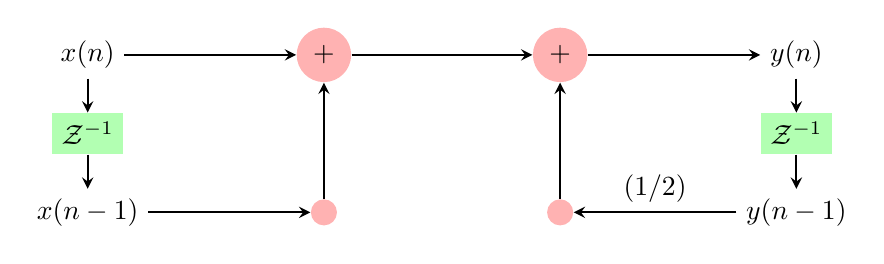
\begin{tikzpicture}
            \node (xn) [rectangle, text centered] {$x(n)$};
            \node (plus0) [circle, fill = red!30, right of = xn, xshift = 2cm] {+};
            \node (z1) [rectangle, below of = xn, fill = green!30] {$\zcal^{-1}$};
            \node (xnlag1) [rectangle, below of = z1] {$x(n-1)$};
            \node (plus1) [circle, fill = red!30, right of = xnlag1, xshift = 2cm] {};
            
            \node (plus3) [circle, fill = red!30, right of = plus0, xshift = 2cm] {+};
            
            \node (yn) [right of = plus3, xshift = 2cm] {$y(n)$};
            \node (z4) [rectangle, below of = yn, fill = green!30] {$\zcal^{-1}$};
            \node (ynlag1) [rectangle, below of = z4] {$y(n-1)$};
            \node (plus4) [circle, fill = red!30, left of = ynlag1, xshift = -2cm] {};
            
            
            \draw [arrow] (xn) -- (plus0);
            \draw [arrow] (xn) -- (z1);
            \draw [arrow] (z1) -- (xnlag1);
            \draw [arrow] (xnlag1) -- (plus1);
            \draw [arrow] (plus1) -- (plus0);
            
            \draw[arrow] (plus0) -- (plus3);
            \draw[arrow] (plus3) -- (yn);
            
            \draw[arrow] (yn) -- (z4);
            \draw[arrow] (z4) -- (ynlag1);
            \draw[arrow] (plus4) -- (plus3);
            \draw[arrow] (ynlag1) -- (plus4) node[midway, above] {$(1/2)$};
        \end{tikzpicture}
    \end{figure}

    Thus, we can represent the system also as $y(n) = \dfrac{1}{2} y(n-1) + x(n) + x(n-1)$.

    \begin{enumerate}
        \item[(a)] Now, we assume that the system is at rest initially, i.e. $y(-n) = 0$ for all $n > 0$. Then, using the equation $y(n) = \dfrac{1}{2} y(n-1) + x(n) + x(n-1)$, we have the first 10 samples of the impulse response as follows (by taking $x(n) = \delta(n)$):
        
        \begin{align*}
            y(0) & = 0.5 y(-1) + \delta(0) + \delta(-1) = 1
            \qquad y(1) = 0.5 y(0) + \delta(1) + \delta(0) = 1.5\\
        \end{align*}

        and for any $n \geq 2$, $\delta(n) = \delta(n-1) = 0$, so,

        $$
        y(n) = \dfrac{1}{2}y(n-1) + \delta(n) + \delta(n-1) = \dfrac{1}{2}y(n-1) = \dots = \dfrac{1}{2^(n-1)} y(1) = \dfrac{3}{2^n} 
        $$

        Thus, the first $10$ samples of the impulse response sequence is 

        $$
        h(n) = \left[ \underset{\uparrow}{1}, \dfrac{3}{2}, \dfrac{3}{4}, \dfrac{3}{8}, \dfrac{3}{16}, \dfrac{3}{32}, \dfrac{3}{64}, \dfrac{3}{128}, \dfrac{3}{256}, \dfrac{3}{512} \right]
        $$

        \item[(b)] The input output relation of the given system is 

        $$
        y(n) = \dfrac{1}{2} y(n-1) + x(n) + x(n-1)
        $$

        Also, since the input output relation of an LTI system is expressed by the discrete convolution of the input sequence with the impulse response sequence, hence

        $$
        y(n) = \sum_{k = -\infty}^\infty x(n-k) h(k) = \sum_{k = 1}^\infty x(n-k) \dfrac{3}{2^{k}} + x(n)
        $$

        since the impulse response function of the system can be compactly expressed as 

        $$
        h(n) = \begin{cases}
            \dfrac{3}{2^n} & n > 0\\
            1 & n = 0
        \end{cases}
        $$

        \item[(c)] With the input sequence $x(n) = [\underset{\uparrow}{1}, 1, 1, 1, \dots]$, and the input output relation as $y(n) = 0.5y(n-1) + x(n) + x(n-1)$, we have 
        
        $$
        y(0) = 0.5 y(-1) + x(0) + x(-1) = 1
        $$

        assuming that the system is at rest initially. Then, for any $n \geq 1$, it follows that $y(n) = 0.5 y(n-1) + 2$, since both $x(n) = x(n-1) = 1$. Thus, we have 

        \begin{align*}
            y(n) 
            & = 2\inv y(n-1) + 2\\
            & = 2\inv[2] y(n-2) + (2\inv + 1) 2\\
            & = 2\inv[3] y(n-3) + (2\inv[2] + 2\inv + 1)2\\
            & = \cdots \\
            & = 2\inv[n] y(0) + 2 (1 + 2\inv + 2\inv[2] + \dots + 2\inv[(n-1)])\\
            & = 2\inv[n] + 2 \dfrac{(1 - 2\inv[n])}{(1 - 2\inv)}\\
            & = 4 - 2\inv[(n-2)] + 2\inv[n] = 4 - 3.2\inv[n], \qquad \forall n \geq 1
        \end{align*}

        Thus, the first 10 samples are given as 

        $$
        \left[ \underset{\uparrow}{1}, 2.5, 3.25, 3.625, 3.8125,
        3.90625,
        3.953125,
        3.9765625,
        3.98828125,
        3.994140625 \right]
        $$


    \end{enumerate}
    
\end{answer}



% Q6
% DONE
\begin{question}
    Consider the discrete time system shown in the following figure.

    \begin{figure}[H]
        \centering
        \includegraphics[width = 0.8\linewidth]{q_figure2.png}
    \end{figure}

    \begin{enumerate}
        \item[(a)] Determine the impulse response.
        \item[(b)] Determine a realization for its inverse system, that is the system which produces $x(n)$ as an output when $y(n)$ is used as an input. 
    \end{enumerate}
\end{question}

\begin{answer}

    The given system can be written as

    $$
    w(n) = 0.8 w(n-1) + x(n), \qquad y(n) = 2w(n) + 3w(n-1)
    $$

    However, using the commutativity of convolution operator, we can represent the given system as shown in the following figure.

    \begin{figure}[H]
        \centering
        \tikzstyle{arrow} = [thick,->,>=stealth]
        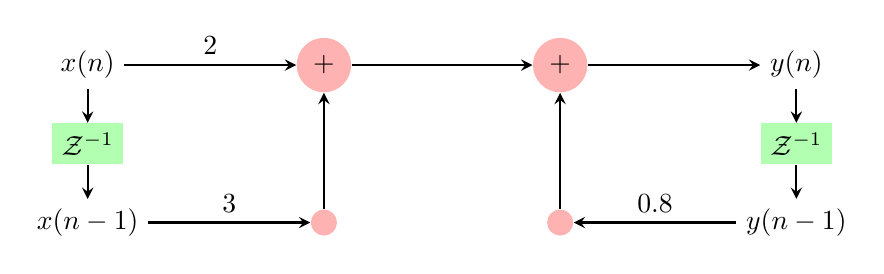
\begin{tikzpicture}
            \node (xn) [rectangle, text centered] {$x(n)$};
            \node (plus0) [circle, fill = red!30, right of = xn, xshift = 2cm] {+};
            \node (z1) [rectangle, below of = xn, fill = green!30] {$\zcal^{-1}$};
            \node (xnlag1) [rectangle, below of = z1] {$x(n-1)$};
            \node (plus1) [circle, fill = red!30, right of = xnlag1, xshift = 2cm] {};
            
            \node (plus3) [circle, fill = red!30, right of = plus0, xshift = 2cm] {+};
            
            \node (yn) [right of = plus3, xshift = 2cm] {$y(n)$};
            \node (z4) [rectangle, below of = yn, fill = green!30] {$\zcal^{-1}$};
            \node (ynlag1) [rectangle, below of = z4] {$y(n-1)$};
            \node (plus4) [circle, fill = red!30, left of = ynlag1, xshift = -2cm] {};
            
            
            \draw [arrow] (xn) -- (plus0) node[midway, above] {$2$};
            \draw [arrow] (xn) -- (z1);
            \draw [arrow] (z1) -- (xnlag1);
            \draw [arrow] (xnlag1) -- (plus1) node[midway, above] {$3$};
            \draw [arrow] (plus1) -- (plus0);
            
            \draw[arrow] (plus0) -- (plus3);
            \draw[arrow] (plus3) -- (yn);
            
            \draw[arrow] (yn) -- (z4);
            \draw[arrow] (z4) -- (ynlag1);
            \draw[arrow] (plus4) -- (plus3);
            \draw[arrow] (ynlag1) -- (plus4) node[midway, above] {$0.8$};
        \end{tikzpicture}
    \end{figure}

    Thus, the difference equation corresponding to the given LTI system is 

    $$
    y(n) = 0.8y(n-1) + 2 x(n) + 3x(n-1)
    $$

    \begin{enumerate}
        \item[(a)] Let, $X(z), Y(z), H(z)$ be the $\zcal$-transformation of the sequences $x(n), y(n)$ and $h(n)$'s respectively. In order to determine the impulse response of the system, we take the $\zcal$-transform to both sides of the above difference equation, which yields 
        
        \begin{align*}
            & Y(z) = 0.8 z\inv Y(z) + 2 X(z) + 3 z\inv X(z)\\
            \Rightarrow \qquad & Y(z)(1 - 0.8z\inv) = X(z) (2 + 3z\inv)\\
            \Rightarrow \qquad & H(z) = \dfrac{Y(z)}{X(z)} = \dfrac{2 + 3z\inv}{1 - 0.8z\inv}\\
            \Rightarrow \qquad & H(z) = -3.75 + \dfrac{5.75}{(1 - 0.8z\inv)}
        \end{align*}

        Thus, inverting the $\zcal$-transform noting that the system is causal since the pole $(0.8)$ lies within the unit circle, we obtain that the impulse response $h(n)$ is given by 

        $$
        h(n) = -3.75\delta(n) + 5.75 (0.8)^n u(n)
        $$

        \item[(b)] The inverse system that produces $x(n)$ as an output when $y(n)$ is used as an input would have a system function given by 
        
        $$
        \widetilde{H}(z) = \dfrac{X(z)}{Y(z)} = \dfrac{1}{H(z)} = \dfrac{(1 - 0.8z\inv)}{(2 + 3z\inv)}
        $$

        And
        
        \begin{align*}
            \widetilde{H}(z)
            & = \dfrac{1}{10} \dfrac{(10 - 8z\inv)}{(2 + 3z\inv)}\\
            & = \dfrac{1}{10} \left[ -\dfrac{8}{3} + \dfrac{(46/3)}{(2 + 3z\inv)} \right]\\
            & = -\dfrac{4}{15} + \dfrac{23}{30} \dfrac{1}{(1 + 1.5z\inv)}
        \end{align*}

        Clearly, the inverse system is anti-causal, and the impulse response would be

        $$
        \widetilde{h}(n) = -\dfrac{4}{15}\delta(n) - \dfrac{23}{30} \left( -\dfrac{3}{2} \right)^n u(-n-1)
        $$

    \end{enumerate}

\end{answer}


% DONE
% Q7

\begin{question}
    Show that any discrete time signal $x(n)$ can be expressed as 
    $$
    x(n) = \sum_{k = -\infty}^{\infty} [x(k) - x(k-1)]u(n-k)
    $$
    where $u(n-k)$ is a unit step delayed by $k$ units in time, that is 
    $$
    u(n-k) = \begin{cases}
        1 & n \geq k\\
        0 & n < k
    \end{cases}
    $$
\end{question}

\begin{answer}
    Consider the following chain of equalities;

    \begin{align*}
        x(n)
        & = \sum_{k = -\infty}^\infty x(k) \delta(n-k) \qquad \text{since, } \delta(n-k) = 1 \text{ iff } n = k\\
        & = \sum_{k = -\infty}^\infty x(k) [u(n-k) - u(n-k-1)] \qquad \text{since, } \delta(r) = u(r) - u(r-1)\\
        & = \sum_{k = -\infty}^\infty x(k)u(n-k) - \sum_{k = -\infty}^\infty x(k)u(n-k-1)\\
        & = \sum_{k = -\infty}^\infty x(k)u(n-k) - \sum_{k' = -\infty}^\infty x(k'-1)u(n-k') \qquad \text{where, } k' = (k+1)\\
        & = \sum_{k = -\infty}^\infty [x(k) - x(k-1)]u(n-k) \qquad \text{since, } k' \text{ is just a dummy variable}
    \end{align*}

    This shows that any discrete time sequence $x(n)$ can be written in the above form.
\end{answer}


% DONE
% Q8
\begin{question}
    Consider the discrete time system shown in the following figure.

    \begin{figure}[H]
        \centering
        \includegraphics[width = 0.8\linewidth]{q_figure3.png}
    \end{figure}

    \begin{enumerate}
        \item[(a)] Determine its impulse response $h(n)$.
        \item[(b)] Show that $h(n)$ is equal to the convolution of the following signals 
        $$
        h_1(n) = \delta(n) + \delta(n-1) \qquad h_2(n) = \left(\frac{1}{2}\right)^n u(n)
        $$  
    \end{enumerate}
\end{question}

\begin{answer}
    \begin{enumerate}
        \item[(a)] The difference equation corresponding to the above discrete time system shown in the question is,

        $$
        y(n) = \dfrac{1}{2} y(n-1) + x(n) + x(n-1)
        $$
    
        Now, denoting $X(z), Y(z)$ and $H(z)$ as the $\zcal$-transform of the discrete time sequence $x(n), y(n)$ and $h(n)$ respectively, and taking $\zcal$-transform on the both sides of the above equation yields
    
        \begin{align*}
            & Y(z) = \dfrac{1}{2} z\inv Y(z) + X(z) + z\inv X(z)\\
            \Rightarrow \qquad & Y(z)(1 - 2\inv z\inv) = X(z)(1 + z\inv)\\
            \Rightarrow \qquad & H(z) = \dfrac{Y(z)}{X(z)} = \dfrac{(1 + z\inv)}{\left(1 - \dfrac{1}{2} z\inv\right)}\\
            \Rightarrow \qquad & H(z) =  \dfrac{1}{\left(1 - \dfrac{1}{2} z\inv\right)} +  \dfrac{z\inv}{\left(1 - \dfrac{1}{2} z\inv\right)}
        \end{align*}
    
        Now, we know that,
    
        \begin{align*}
            \zcal\{  2^n u(n) \} = \dfrac{1}{\left(1 - \dfrac{1}{2} z\inv\right)} \qquad \text{with ROC }  \vert z \vert > 1/2
        \end{align*}
    
        and using the properties of $\zcal$-transform it follows that, 
    
        $$
        h(n) = \zcal\inv\{ H(z)\} = 2\inv[n] u(n) + 2\inv[(n-1)] u(n-1)
        $$

        assuming that the system is causal.
        
    \item[(b)] Let us consider the convolution of the sequences $h_1(n)$ and $h_2(n)$. 
    
    \begin{align*}
        (h_1 \ast h_2) (n)
        & = \sum_{k = -\infty}^{\infty} h_1(n - k) h_2(k)\\
        & = \sum_{k = -\infty}^{\infty} (\delta(n-k) + \delta(n-k-1)) (1/2)^k u(k)\\
        & = \sum_{k = -\infty}^{\infty} \delta(n-k) (1/2)^k u(k) + \sum_{k = -\infty}^{\infty} \delta(n-k-1) (1/2)^k u(k)\\
        \text{Since, } \delta(r) = 1 \text{ iff } r = 0, & \text{ and is otherwise 0, we have, }\\
        & = (1/2)^n u(n) + (1/2)^{(n-1)} u(n-1)\\
        & = h(n)
    \end{align*}

    \end{enumerate}
\end{answer}


% DONE
% Q9
\begin{question}
    Express the $z$-transform of $y(n) = \sum_{k = -\infty}^n x(k)$ in terms of $X(z)$.
\end{question}

\begin{answer}
    Note that,
    $$
    y(n) = \sum_{k = -\infty}^n x(k) = \sum_{k = -\infty}^\infty x(k)u(n-k) = x(n) \ast u(n)
    $$

    since $u(n - k)$ takes value $1$ if and only if $k \leq n$, and is otherwise equal to $0$, and $\ast$ denotes the discrete convolution operator.
    
    Now, we know that the $\zcal$-transform of $u(n)$ is $(1 - z\inv)\inv$ with ROC $\{ z : \vert z \vert > 1 \}$. And we also know that the discrete convolution in time domain becomes multiplication in $\zcal$-domain. Hence,

    \begin{align*}
        Y(z) 
        & = \zcal\{ y(n)\} = \zcal\{ u(n) \ast x(n) \}\\
        & = \zcal\{ u(n) \} \zcal\{ x(n) \}\\
        & = \dfrac{1}{(1 - z\inv)} X(z)    
    \end{align*}

    with the ROC $A \cap \{ z : \vert z \vert > 1\}$, where $A$ is the ROC of the $\zcal$-transform of $x(n)$ i.e. of $X(z)$.
\end{answer}

% DONE
% Q10

\begin{question}
    Compute the convolution of the following signals by means of the $\zcal$-transform
    $$
    x_1(n) = \begin{cases}
        3^{(-n)} & n \geq 0\\
        2^n & n < 0\\
    \end{cases},\qquad 
    x_2(n) = 2^{(-n)} u(n)
    $$
\end{question}

\begin{answer}
    First, we note that,

    $$
    X_2(z) = \zcal\{ x_2(n)\} = \dfrac{1}{(1 - 2\inv z\inv)}
    $$

    with ROC $\{ z : \vert z \vert > 1/2\}$, and

    \begin{align*}
        X_1(z) 
        & = \zcal\{ x_1(n) \} \\
        & = \sum_{n = -\infty}^{\infty} x_1(n)z\inv[n]\\
        & = \sum_{n = -\infty}^{(-1)} 2^n z\inv[n] + \sum_{n = 0}^{\infty} 3\inv[n] z\inv[n]\\
        & = \dfrac{2\inv z}{(1 - 2\inv z)} + \dfrac{1}{(1 - 3\inv z\inv)}\\
        & = \dfrac{1}{(2 z\inv - 1)} + \dfrac{1}{(1 - 3\inv z\inv)}\\
    \end{align*}

    with ROC $\{ z : (1/3) < \vert z \vert < 2 \}$. Since discrete convolution in time domain becomes multiplication in $\zcal$-domain, we have 

    \begin{align*}
        X_1(z)X_2(z)
        & = \dfrac{1}{(1 - (1/2) z\inv)(2 z\inv - 1)} + \dfrac{1}{(1 - (1/2) z\inv)(1 - (1/3) z\inv)}\\
        & = \dfrac{(1/3)}{(1 - (1/2) z\inv)} + \dfrac{(4/3)}{(2z\inv - 1)} + \dfrac{3}{(1 - (1/2) z\inv)} + \dfrac{(-2)}{(1 - (1/3) z\inv)}\\
        & = \dfrac{(10/3)}{(1 - (1/2) z\inv)} - \dfrac{(4/3)}{(1 - 2z\inv)} - \dfrac{2}{(1 - (1/3) z\inv)}
    \end{align*}

    Therefore,

    \begin{align*}
        x_1(n) \ast x_2(n)
        & = \zcal\inv\{ X_1(z)X_2(z) \}\\
        & = \zcal\inv\left\{ \dfrac{(10/3)}{(1 - (1/2) z\inv)} - \dfrac{(4/3)}{(1 - 2z\inv)} - \dfrac{2}{(1 - (1/3) z\inv)} \right\}\\
        & = \left[ \dfrac{10}{3} \left( \dfrac{1}{2} \right)^n - 2 \left( \dfrac{1}{3} \right)^n \right]u(n) + \left(\dfrac{4}{3}\right) 2^n u(-n-1)
    \end{align*}

    since the term $\dfrac{(4/3)}{(1 - 2z\inv)}$ is due to an anti-causal discrete time signal.

\end{answer}


% DONE
% Q11

\begin{question}
    Apply the final value theorem to determine $x(\infty)$ for the signal 
    $$x(n) = \begin{cases}
        1 & \text{if } n \text{ is even}\\
        0 & \text{otherwise}
    \end{cases}$$
\end{question}

\begin{answer}
    Let us first apply the one-sided $\zcal$-transform on $x(n)$.

    \begin{align*}
        \zcal^+\{ x(n) \}
        & = \sum_{n = 0}^\infty x(n) z\inv[n]\\
        & = \sum_{\substack{n = 0 \\ n \text{ is even}}}^\infty z\inv[n] \qquad \text{since, } x(n) = 1 \text{ iff } n \text{ is even}\\
        & = 1 + z\inv[2] + z\inv[4] + \ldots \infty\\
        & = \dfrac{1}{(1 - z\inv[2])}
    \end{align*}

    According to final value theorem,

    \begin{align*}
        x(\infty)
        & = \lim_{z \rightarrow 1} (z - 1) \zcal^+ \{ x(n)\}\\
        & = \lim_{z \rightarrow 1} (z - 1) \dfrac{1}{(1 - z\inv)(1 + z\inv)}\\
        & = \lim_{z \rightarrow 1} (z - 1) \dfrac{z}{(z - 1)(1 + z\inv)}\\
        & = \lim_{z \rightarrow 1} \dfrac{z}{(1 + z\inv)}=  \dfrac{1}{2}
    \end{align*}

    Hence, $x(\infty) = (1/2)$.
\end{answer}

% Q12
% DONE
\begin{question}
    Determine the causal signal $x(n)$ having the $\zcal$-transform 
    $$
    X(z) = \dfrac{1}{(1 - 2z^{(-1)})(1 - z^{(-1)})^2}
    $$
\end{question}


\begin{answer}
    Note that,

    \begin{align*}
        X(z)
        & = \dfrac{1}{(1 - 2z^{(-1)})(1 - z^{(-1)})^2}\\
        & = \dfrac{2(1 - z\inv) - (1 - 2z\inv)}{(1 - 2z\inv)(1 - z\inv)^2}\\
        & = \dfrac{2}{(1 - 2z\inv)(1 - z\inv)} - \dfrac{1}{(1 - z\inv)^2}\\
        & = 2 \left[ \dfrac{2(1 - z\inv) - (1 - 2z\inv)}{(1 - 2z\inv)(1 - z\inv)} \right] - \dfrac{1}{(1 - z\inv)^2}\\
        & = \dfrac{4}{(1 - 2z\inv)} - 2 \dfrac{1}{(1 - z\inv)} + \dfrac{1}{(1 - z\inv)^2}
    \end{align*}

    Now, we know that, $\zcal\{ a^n u(n) \} = \dfrac{1}{(1 - az\inv)}$, and by differentiation in $\zcal$-domain, $\zcal\{ a^n n u(n) \} = \dfrac{az\inv}{(1 - a z\inv)^2}$. Now, introducing a lag of $(-1)$ in the system, 

    $$
    \zcal\{ a^{(n+1)}(n+1)u(n+1) \} = \dfrac{a}{(1 - az\inv)^2}
    $$

    In view of this, and since the given sequence $x(n)$ is causal, inverting the $\zcal$-transformation $X(z)$, we obtain

    $$
    x(n) = (2^{(n+2)} - 2) u(n) + (n+1) u(n+1)
    $$

\end{answer}


% Q13
% DONE
\begin{question}
    Let, $x(n)$ be a sequence with $\zcal$-transform $X(z)$. Determine, in terms of $X(z)$, the $\zcal$-transforms of the following signals.
    \begin{enumerate}
        \item[(a)] $x_1(n) = \begin{cases}
            x(n/2) & \text{if } n \text{ is even}\\
            0 & \text{otherwise}
        \end{cases}$
        \item[(b)] $x_2(n) = x(2n)$.
    \end{enumerate}
\end{question}

\begin{answer}
    \begin{enumerate}
        \item[(a)] The $\zcal$-transform of the given signal $x_1(n)$ is,
        
        \begin{align*}
            X_1(z) 
            & = \zcal\{ x_1(n) \}\\
            & = \sum_{n = -\infty}^\infty x_1(n)z\inv[n]\\
            & = \sum_{\substack{n = -\infty\\ n \text{ is even}}}^\infty x(n/2) z\inv[n]\\
            & = \sum_{m = -\infty}^\infty x(m) z\inv[2m] \qquad \text{where, } n = 2m, \text{ with } m \in \Z\\
            & = \sum_{m = -\infty}^\infty x(m) (z^2)\inv[m]
            = X(z^2)
        \end{align*}

        where $X(z)$ is the $\zcal$-transform of $x(n)$. Therefore, $X_1(z) = X(z^2)$.

        \item[(b)] We start by noting that $\zcal$-transform of $x(n)$ is given as
        
        $$
        X(z) = \sum_{n = -\infty}^{\infty} x(n)z\inv[n]
        $$

        Hence, $X(-z) = \sum_{n = -\infty}^{\infty} x(n)(-z)\inv[n] = \sum_{n = -\infty}^{\infty} (-1)^n x(n)z\inv[n]$. Summing these two yields,

        \begin{align*}
            X(z) + X(-z)
            & = \sum_{n = -\infty}^{\infty} x(n) (1 + (-1)^n) z\inv[n]\\
            & = \sum_{m = -\infty}^{\infty} 2 \times x(2m) z\inv[2m] \qquad \text{ where, } n = 2m, \text{ and all odd order terms will cancel}\\
            & = 2 \sum_{m = -\infty}^{\infty} x_2(m) (z^2)\inv[m]\\
            & = \zcal\{ x_2(n) \} (z^2)
        \end{align*}

        Hence,
        $$
        X_2(z) = \zcal\{ x_2(n) \}(z) = \dfrac{1}{2} \left[X(\sqrt{z}) + X(-\sqrt{z}) \right]
        $$

    \end{enumerate}
\end{answer}

% Q14
% DONE
\begin{question}
    Determine the signal $x(n)$ with $\zcal$-transform 
    $$
    X(z) = e^z + e^{(1/z)} \qquad \vert z \vert \neq 0
    $$
\end{question}

\begin{answer}
    We have $X(z)$ as the $\zcal$-transform of the discrete time signal $x(n)$. Note that

    \begin{align*}
        X(z)
        & = e^z + e^{(1 / z)}\\
        & = \sum_{n = 0}^{\infty} \dfrac{z^n}{n!} + \sum_{n = 0}^{\infty} \dfrac{1}{z^n n!} \qquad \text{ by infinite Taylor series expansion of } e^z\\
        & = \sum_{m = -\infty}^{0} \dfrac{z\inv[m]}{(-m)!} + \sum_{n = 0}^{\infty} \dfrac{z\inv[n]}{n!} \qquad \text{where, } m = (-n)\\
        & = 2 + \sum_{m = -\infty}^{(-1)} \dfrac{z\inv[m]}{(-m)!} + \sum_{n = 1}^{\infty} \dfrac{z\inv[n]}{n!}, \qquad \text{taking the constant term apart}
    \end{align*}

    Hence, the discrete time signal $x(n)$ is given by,

    $$
    x(n) = \begin{cases}
        2 & \text{ if } n = 0\\
        \dfrac{1}{\vert n \vert !} & \text{ if } n \neq 0\\
    \end{cases}
    $$

    where $\vert n \vert$ denotes the absolute value of $n$.
\end{answer}


% Q15
% DONE
\begin{question}
    Determine the signal $x(n)$ with $z$-transform
    $$
    X(z) = \dfrac{3}{1 - (10/3)z^{(-1)} + z^{(-2)}}
    $$
    if $X(z)$ converges on the unit circle.
\end{question}

\begin{answer}
    Note that,
    $$
    X(z) = \dfrac{3}{(1 - 3z\inv)\left(1 - \dfrac{1}{3}z\inv \right)}
    $$

    The two poles of $X(z)$ are $z = \dfrac{1}{3}$ and $z = 3$ respectively, and since the $\zcal$-transform $X(z)$ converges on the unit circle, it must have the ROC of the form, 

    $$
    ROC = \{ z : \dfrac{1}{3} < r_1 \leq \vert z \vert \leq r_2 < 3 \}
    $$

    for some $r_1, r_2 > 0$. Now observe that, the given $X(z)$ can be decomposed as

    $$
    X(z) = \dfrac{27/8}{(1 - 3z\inv)} - \dfrac{3/8}{\left( 1 - \dfrac{1}{3} z\inv \right)}
    $$

    However, since the ROC includes the unit circle, the first term in $X(z)$ i.e. $\dfrac{1}{(1 - 3z\inv)}$ with a pole at $z = 3$ must be due to an anti-causal part. Whereas, the second term in $X(z)$ i.e. $\dfrac{1}{(1 -3\inv z\inv)}$ with a pole at $(1/3)$ is due to the causal part. Therefore,

    $$
    \zcal\inv\{ \dfrac{1}{(1 - 3z\inv)} \} = (-3)^n u(-n-1) \qquad 
    \zcal\inv\{ \dfrac{1}{(1 - 3\inv z\inv)} \} = 3\inv[n] u(n)
    $$

    Thus, we have the required signal $x(n)$ given by 

    $$
    x(n) = \dfrac{27}{8} (-3)^n u(-n-1) - \dfrac{3}{8} \left(\dfrac{1}{3}\right)^n u(n), \qquad n = 0, \pm 1, \pm 2, \dots 
    $$
\end{answer}


% Q16
% DONE
\begin{question}
    Consider the system 
    $$
    H(z) = \dfrac{(1 - 2z^{(-1)} + 2z^{(-2)} - z^{(-3)})}{(1 - z^{(-1)})(1 - 0.5 z^{(-1)})(1 - 0.2z^{(-1)}) } \qquad \text{ROC: } 0.5 < \vert z \vert < 1
    $$
    \begin{enumerate}
        \item[(a)] Sketch the pole zero pattern. Is the system stable?
        \item[(b)] Determine the impulse response of the system.
    \end{enumerate}
\end{question}

\begin{answer}
    \begin{enumerate}
        \item[(a)]
        
        First we start by factorizing the numerator of the system function $H(z)$.

        \begin{align*}
            (1 - 2z\inv + 2z\inv[2] - z\inv[3])
            & = (1 - 3z\inv + 3z\inv[2] - z\inv[3]) + (z\inv - z\inv[2])\\
            & = (1 - z\inv)^3 + z\inv (1 - z\inv)\\
            & = (1 - z\inv) (1 - z\inv + z\inv[2])\\
            & = (1 - z\inv)(1 + \omega z\inv)(1 + \omega^2 z\inv)        
        \end{align*}

        where the last line follows from that $(\omega + \omega^2) = (-1)$, where $\omega$ is a complex cube root of unity except $1$.

        Since the ROC does not include $z = 1$, we have

        \begin{align*}
            H(z) 
            & = \dfrac{(1 + \omega z\inv)(1 + \omega^2 z\inv)}{(1 - 0.5z\inv)(1 - 0.2z\inv)}\\
            & = \dfrac{(z + \omega)(z + \omega^2)}{(z - 0.5)(z - 0.2)}            
        \end{align*}

        In other words, the two poles of the system function are $0.2$ and $0.5$ and the two zeros of the system function are $\left( \dfrac{1 - \sqrt{3}j }{2} \right)$ and $\left( \dfrac{1 + \sqrt{3}j }{2} \right)$, where $j$ is the imaginary number satisfying $(j^2 + 1) = 0$. Since the ROC of the system does not contain the unit circle, the system is not BIBO stable.

        \item[(b)] Note that, 
        
        \begin{align*}
            H(z) 
            & = \dfrac{(z^2 - z + 1)}{(z - 0.5)(z - 0.2)}\\
            & = \dfrac{(1 - z\inv + z\inv[2])}{(1 - 0.5 z\inv)(1 - 0.2z\inv)}\\
            & = 10 + \dfrac{(-9) + 6z\inv}{(1 - 0.5z\inv)(1 - 0.2z\inv)}\\
            & = 10 + \dfrac{5}{(1 - 0.5z\inv)} - \dfrac{14}{(1 - 0.2z\inv)}
        \end{align*}

        Since, both the poles $0.2$ and $0.5$ are less than $1$ in magnitude and the ROC is specified by $\vert z \vert > 0.5$, the impulse response function is causal. Hence, by inverting the $\zcal$-transform, we obtain that 

        $$
        h(n) = 10\delta(n) + 5 (0.5)^n u(n) - 14 (0.2)^n u(n)
        $$

        where 

        $$
        \delta(n) = \begin{cases}
            1 & n = 0\\
            0 & n \neq 0
        \end{cases},
        \qquad
        u(n) = \begin{cases}
            1 & n > 0\\
            0 & n \leq 0
        \end{cases}
        $$

    \end{enumerate}
\end{answer}



% Q17
% DONE
\begin{question}
    Determine the response $y(n)$, $n \geq 0$, of the system described by the second order difference equation 
    $$
    y(n) - 3y(n-1) - 4y(n-2) = x(n) + 2 x(n-1)
    $$
    to the input $x(n) = 4^n u(n)$.
\end{question}

\begin{answer}
    Let, $X(z)$ and $Y(z)$ denote the $\zcal$-transform of the input sequence $x(n)$ and the output sequence $y(n)$ respectively. 

    Clearly, as $x(n) = 4^n u(n)$,

    $$
    X(z) = \dfrac{1}{(1 - 4 z\inv)}
    $$

    with ROC $\{ z : \vert z \vert > (1/4) \}$. Now taking $\zcal$-transform to both sides of the second order difference equation 

    \begin{align*}
        & Y(z) - 3 z\inv Y(z) - 4 z\inv[2] Y(z) = X(z) + 2 z\inv X(z)\\
        \Rightarrow \qquad & Y(z) (1 - 3z\inv - 4z\inv[2]) = (1 + 2z\inv) \dfrac{1}{(1 - 4z\inv)}\\
        \Rightarrow \qquad & Y(z) = \dfrac{(1 + 2z\inv)}{(1 - 4z\inv)(1 - 3z\inv - 4z\inv[2])}\\
        \Rightarrow \qquad & Y(z) = \dfrac{(1 + 2z\inv)}{(1 - 4z\inv)^2(1 + z\inv)}\\
        \Rightarrow \qquad & Y(z) = \dfrac{(-4/25)}{(1 - 4z\inv)} + \dfrac{6/5}{(1 - 4z\inv)^2} + \dfrac{(-1/25)}{(1 + z\inv)}\\
    \end{align*}

    Now, it follows that

    \begin{align*}
        & \zcal\{ 4^n u(n) \} = \dfrac{1}{(1 - 4z\inv)}\\
        \Rightarrow \qquad & \zcal\{ n4^n u(n) \} = \dfrac{4z\inv}{(1 - 4z\inv)^2} \qquad \text{by differentiation in } \zcal \text{-domain}\\
        \Rightarrow \qquad & \zcal\{ (n+1)4^{n}u(n+1) \} = \dfrac{1}{(1 - 4z\inv)^2}
    \end{align*}

    Thus, inverting the $\zcal$-transform and assuming that the output of the system is a causal sequence, we obtain

    $$
    y(n) = \dfrac{(-4)}{25} 4^n u(n) + \dfrac{6}{5} (n+1) 4^n u(n+1) - \dfrac{1}{25} (-1)^n u(n)
    $$

\end{answer}



% Q18

\begin{question}
    Two signals $s(n)$ and $v(n)$ are related through the following difference equations
    $$
    s(n) + a_1 s(n-1) + \dots + a_N s(n-N) = b_0 v(n)
    $$
    Design the block diagram realization of:
    \begin{enumerate}
        \item[(a)] The system that generates $s(n)$ when excited by $v(n)$.
        \item[(b)] The system that generates $v(n)$ when excited by $s(n)$.
        \item[(c)] What is the impulse response of the cascade interconnection of systems in parts (a) and (b)?
    \end{enumerate}
\end{question}


\begin{answer}
    \begin{enumerate}
        \item[(a)] We can rewrite the equation as 
        
        $$
        s(n) = -a_1 s(n-1) - a_2s(n-2) - \dots - a_N s(n-N) + b_0 v(n)
        $$
        
        The design of the system is as follows:
        
        \begin{figure}[H]
            \centering
            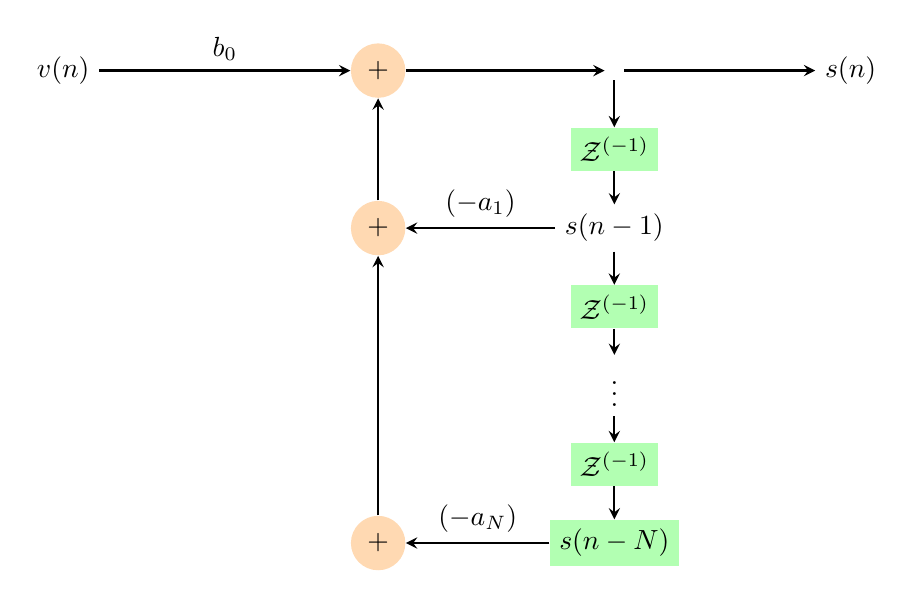
\begin{tikzpicture}
                \node (vn) [rectangle, text centered] {$v(n)$};
                \node (join1) [circle, fill = orange!30, right of = vn, xshift = 3cm] {+};
                \node (sn) [rectangle, text centered, right of = join1, xshift = 2cm] {};
                \node (snout) [rectangle, text centered, right of = sn, xshift = 2cm] {$s(n)$};
                
                \node (z1) [rectangle, fill = green!30, text centered, below of = sn] {$\zcal\inv$};
                \node (snlag1) [rectangle, text centered, below of = z1] {$s(n-1)$};
                \node (z2) [rectangle, fill = green!30, text centered, below of = snlag1] {$\zcal\inv$};
                \node (dots) [rectangle, text centered, below of = z2] {$\vdots$};
                \node (z3) [rectangle, fill = green!30, text centered, below of = dots] {$\zcal\inv$};
                \node (snlagn) [rectangle, fill = green!30, text centered, below of = z3] {$s(n-N)$};
                \node (join2) [circle, fill = orange!30, left of = snlag1, xshift = -2cm] {+};
                \node (join3) [circle, fill = orange!30, left of = snlagn, xshift = -2cm] {+};                
                
                
                \draw [arrow] (vn) -- (join1) node[midway, above] {$b_0$};
                \draw [arrow] (join1) -- (sn);
                \draw [arrow] (sn) -- (z1);
                \draw [arrow] (z1) -- (snlag1);
                \draw [arrow] (snlag1) -- (z2);
                \draw [arrow] (z2) -- (dots);
                \draw [arrow] (dots) -- (z3);
                \draw [arrow] (z3) -- (snlagn);
                \draw [arrow] (snlag1) -- (join2) node[midway, above] {$(-a_1)$};
                \draw [arrow] (snlagn) -- (join3) node[midway, above] {$(-a_N)$};
                \draw [arrow] (join3) -- (join2);
                \draw [arrow] (join2) -- (join1);
                \draw [arrow] (sn) -- (snout);
            \end{tikzpicture}
        \end{figure}
        
        \item[(b)] The system which generates $v(n)$ when excited by $s(n)$ can be obtained from the above equation as;
        
        $$
        v(n) = \dfrac{1}{b_0} s(n) + \dfrac{a_1}{b_0}s(n-1) + \dots + \dfrac{a_N}{b_0} s(n-N)
        $$

        This can be implementated by the following network shown in the figure.

        \begin{figure}[H]
            \centering
            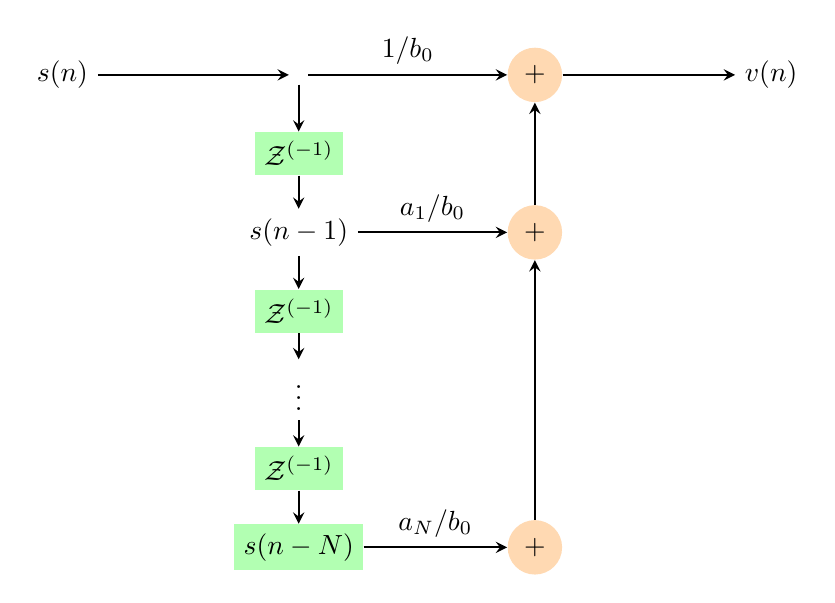
\begin{tikzpicture}
                \node (vn) [rectangle, text centered] {$s(n)$};
                \node (sn) [rectangle, text centered, right of = vn, xshift = 2cm] {};
                \node (join1) [circle, fill = orange!30, right of = sn, xshift = 2cm] {+};
                \node (snout) [rectangle, text centered, right of = join1, xshift = 2cm] {$v(n)$};
                \node (z1) [rectangle, fill = green!30, text centered, below of = sn] {$\zcal\inv$};
                \node (snlag1) [rectangle, text centered, below of = z1] {$s(n-1)$};
                \node (z2) [rectangle, fill = green!30, text centered, below of = snlag1] {$\zcal\inv$};
                \node (dots) [rectangle, text centered, below of = z2] {$\vdots$};
                \node (z3) [rectangle, fill = green!30, text centered, below of = dots] {$\zcal\inv$};
                \node (snlagn) [rectangle, fill = green!30, text centered, below of = z3] {$s(n-N)$};
                \node (join2) [circle, fill = orange!30, right of = snlag1, xshift = 2cm] {+};
                \node (join3) [circle, fill = orange!30, right of = snlagn, xshift = 2cm] {+};                
                
                \draw [arrow] (vn) -- (sn);
                \draw [arrow] (sn) -- (join1) node[midway, above] {$1/b_0$};
                \draw [arrow] (sn) -- (z1);
                \draw [arrow] (z1) -- (snlag1);
                \draw [arrow] (snlag1) -- (z2);
                \draw [arrow] (z2) -- (dots);
                \draw [arrow] (dots) -- (z3);
                \draw [arrow] (z3) -- (snlagn);
                \draw [arrow] (snlag1) -- (join2) node[midway, above] {$a_1 / b_0$};
                \draw [arrow] (snlagn) -- (join3) node[midway, above] {$a_N / b_0$};
                \draw [arrow] (join3) -- (join2);
                \draw [arrow] (join2) -- (join1);
                \draw [arrow] (join1) -- (snout);
            \end{tikzpicture}
        \end{figure}
        
        \item[(c)] To obtain the impulse response of the cascade connection between the systems in parts (a) and (b), we compute the system function for both these systems.
        
        Now starting with the difference equation and applying the $\zcal$-transform, denoting the $\zcal$-transformation of $s(n), v(n)$ as $S(z)$ and $V(z)$ respectively, we obtain,

        \begin{align*}
            & S(z) + a_1 z\inv S(z) + \dots + a_N z\inv[N] S(z) = b_0 V(z)\\
            \Rightarrow \qquad & S(z) ( 1 + a_1 z\inv + \dots + a_N z\inv[N]) = b_0 V(z)\\
            \text{Hence, } & \text{ the system function in part (a) is,}\\
            & H_1(z) = \zcal\{ h_1(n)\} = \dfrac{S(z)}{V(z)} = \dfrac{1}{( 1 + a_1 z\inv + \dots + a_N z\inv[N])}\\
            \text{whereas, } & \text{ the system function in part (b) is,}\\
            & H_2(z) = \zcal\{ h_2(n)\} = \dfrac{V(z)}{S(z)} = ( 1 + a_1 z\inv + \dots + a_N z\inv[N])\\
        \end{align*}

        Since, the cascade connection has impulse response function given by $(h_1\ast h_2)(n)$, it follows that the system function of the cascade connection of the two systems is $H_1(z)H_2(z)$, and $H_1(z)H_2(z) = 1$. Thus, the impulse response of the cascade interconnection of those system is simply $\zcal\inv\{ 1 \} = \delta(n)$.


    \end{enumerate}
\end{answer}


% Q19
\begin{question}
    Consider a discrete time LTI system described by the following input-output relation:
    $$
    y(n) = ay(n-1) + x(n) - \dfrac{1}{a} x(n-1)
    $$
    \begin{enumerate}
        \item[(a)] Determine a closed form expression for the impulse response $h(n)$ of this system (in terms of $a$).
        \item[(b)] Determine a closed form expression for the autocorrelation sequence $r_{hh}(n)$ corrsponding to the impulse response of the system.
        \item[(c)] The signal below is input to the system above.
        $$
        x(n) = \dfrac{\sin (3\pi n / 4)}{\pi n}
        $$   
        \begin{enumerate}
            \item[(i)] Plot the energy density spectrum for the output $y(n)$.
            \item[(ii)] Find the total energy in $y(n)$ (in terms of $a$). 
        \end{enumerate}
    \end{enumerate}
\end{question}

\begin{answer}
    \begin{enumerate}
        \item[(a)] Let, $X(z)$ and $Y(z)$ be the $\zcal$-transformation of $x(n)$ and $y(n)$ respectively. Then, taking $\zcal$-transformation on the both sides of the above equation yields
        
        \begin{align*}
            & Y(z) = az\inv Y(z) + X(z) - a\inv z\inv X(z)\\
            \Rightarrow \qquad & Y(z) (1 - az\inv) = X(z) (1 - a\inv z\inv)\\
            \Rightarrow \qquad & H(z) = \dfrac{Y(z)}{X(z)} = \dfrac{(1 - a\inv z\inv)}{(1 - az\inv)}, \qquad \text{where } H(z) \text{ is the system function}\\
            \Rightarrow \qquad & H(z) = \dfrac{1}{a^2} + \dfrac{(1 - a\inv[2])}{(1 - az\inv)} 
        \end{align*}

        Thus, by inverting the $\zcal$-transform (assuming that the system is causal) we obtain that 

        $$
        h(n) = \dfrac{1}{a^2} \delta(n) + \left(1 - \dfrac{1}{a^2} \right) a^n u(n), \qquad n = 0, \pm 1, \pm 2, \dots
        $$

        \item[(b)] Let $r_{hh}(n)$ be the autocorrelation sequence corresponding to the impulse response of the system and let $R(z)$ is the $\zcal$-transformation of this autocorrelation sequence. Then, we know that $R(z) = H(z)H(z\inv)$, hence 
        
        \begin{align*}
            R(z) 
            & = H(z)H(z\inv)\\
            & = \dfrac{(1 - a\inv z\inv)}{(1 - az\inv)} \times \dfrac{(1 - a\inv z)}{(1 - a z)}\\
            & = \dfrac{(z - a\inv)}{(z - a)} \times \dfrac{(1 - a\inv z)}{(1 - a z)}\\
            & = \dfrac{a\inv (az - 1)}{a(a\inv z - 1)} \times \dfrac{(1 - a\inv z)}{(1 - a z)}\\
            & = a\inv[2]       
        \end{align*}

        Thus, the autocorrelation sequence $r_{hh}(n) = a\inv[2] \delta(n)$, where $\delta(n)$ is the impulse response sequence.

        \item[(c)] We start by noting that
        
        \begin{align*}
            x(n)
            & = \dfrac{\sin(3\pi n /4)}{\pi n}\\
            & = \dfrac{1}{2j \pi n} \left[ e^{j \frac{3\pi}{4}n } - e^{-j \frac{3\pi}{4}n } \right]\\
            & = \dfrac{1}{2j \pi n} \times jn \int_{-3\pi/4}^{3\pi/4} e^{j \omega n} d\omega\\
            & = \dfrac{1}{2\pi} \int_{-\pi}^{\pi} X(\omega) e^{j \omega n} d\omega
        \end{align*}

        where 

        $$
        X(\omega) = \begin{cases}
            1 & \text{ if } \vert \omega \vert \leq \dfrac{3\pi}{4}\\
            0 & \text{ otherwise}
        \end{cases}
        $$

        Thus, the given signal $x(n)$ is the inverse DTFT of $X(\omega)$, hence $X(\omega)$ is the DTFT of $x(n)$. Now, taking DTFT on both sides of the given LTI system, we obtain that 

        \begin{align*}
            & Y(\omega) = a e^{-j\omega} Y(\omega) + X(\omega) - \dfrac{1}{a} e^{-j\omega} X(\omega)\\
            \Rightarrow \qquad & Y(\omega) = X(\omega) \dfrac{(1 - a\inv e^{-j\omega})}{(1 - a e^{-j\omega})}\\
            \Rightarrow \qquad & \vert Y(\omega) \vert^2 = \vert X(\omega) \vert^2 \left\vert \dfrac{(1 - a\inv e^{-j\omega})}{(1 - a e^{-j\omega})} \right\vert^2\\
            \Rightarrow \qquad & \vert Y(\omega) \vert^2 = \vert X(\omega) \vert^2 \dfrac{(1 - a\inv e^{-j\omega})(1 - a\inv e^{j\omega})}{(1 - ae^{-j\omega})(1 - ae^{j\omega})} \\
            \Rightarrow \qquad & \vert Y(\omega) \vert^2 = \vert X(\omega) \vert^2 \dfrac{(1 + a\inv[2] - 2a\inv \cos(\omega))}{(1 + a^2 - 2a \cos(\omega))}\\
            \Rightarrow \qquad & \vert Y(\omega) \vert^2 = \vert X(\omega) \vert^2 \dfrac{1}{a^2} \dfrac{(a^2 + 1 - 2a \cos(\omega))}{(1 + a^2 - 2a \cos(\omega))}\\
            \Rightarrow \qquad & \vert Y(\omega) \vert^2 = \vert X(\omega) \vert^2 \dfrac{1}{a^2}\\
        \end{align*}

        Thus, 

        $$
        \vert Y(\omega) \vert^2
        = \begin{cases}
            a\inv[2] & \text{ if } \vert \omega \vert \leq \frac{3\pi}{4}\\
            0 & \text{ otherwise }
        \end{cases}
        $$

        The plot of this energy spectral density of the output is given in the following figure.

        \begin{figure}[H]
            \centering
            \includegraphics[width = 0.7\linewidth]{energy.png}
        \end{figure}

        The total energy in $y(n)$ is,

        \begin{align*}
            E_{yy}
            & = \sum_{n = -\infty}^{\infty} \vert y(n)\vert^2\\
            & = \dfrac{1}{2\pi} \int_{\pi}^{\pi} \vert Y(\omega) \vert^2 d\omega\\
            & = \dfrac{1}{2\pi} \int_{3\pi/4}^{3\pi/4} a\inv[2] d\omega\\
            & = a\inv[2] \dfrac{3\pi / 2}{2\pi} = \dfrac{3}{4a^2}
        \end{align*}
    \end{enumerate}
\end{answer}




% Q20
\begin{question}
    \begin{enumerate}
        \item[(a)] Consider the analog signal $x_a(t) = 3 \cos(100 \pi t)$. 
        \begin{enumerate}
            \item[(i)] Determine the minimum sampling rate required to avoid aliasing.
            \item[(ii)] Suppose that the signal is sampled at the rate $F_s = 200 Hz$. What is the discrete time signal obtained after sampling?
        \end{enumerate}
        \item[(b)] Show that the fundamental period $N_p$ of the signals $s_k(n) - e^{j 2\pi kn/N}$ for $k = 0, 1, 2, \dots$ is given by $N_p = N / GCD(k, N)$, where GCD is the greatest common divisor. What is the fundamental period of this set for $N = 7$ and $16$? 
    \end{enumerate}
\end{question}


\begin{answer}
    \begin{enumerate}
        \item[(a)] 
        \begin{enumerate}
            \item[(i)] We have $x_a(t) = 3\cos(100 \pi t)$, hence the frequency of the signal is $f = 50 Hz$. By Nyquist Sampling theorem, it follows that we need the sampling rate to be at least twice as large as the frequency of the analog signal to avoid aliasing. Hence, the minimum sampling rate required is $(2 \times 50) = 100 Hz$, i.e. $100$ samples per second.
            \item[(ii)] Since the signal is sampling at the rate $F_s = 200 Hz$, hence there are $200$ samples taken per second. Assuming the samples taken are equispaced in the time domain, the sampling is done at the time $t = 0, \dfrac{1}{200}, \dfrac{2}{200}, \dfrac{3}{200}, \dots$. Hence, the discrete time signal obtained would be 
            $$
            x(n) = x_a\left(\dfrac{n}{200}\right) = 3 \cos\left( 100 \pi \dfrac{n}{200} \right) = 3 \cos\left( \dfrac{n\pi}{2} \right), \qquad n = 0, \pm 1, \pm 2, \dots
            $$ 

            This can be rewritten as,

            $$
            x(n) = \begin{cases}
                1 & n = 0, \pm 4, \pm 8, \dots\\
                (-1) & n = \pm 2, \pm 6, \pm 10, \dots\\
                0 & \text{otherwise}
            \end{cases}
            $$

        \end{enumerate} 
        \item[(b)] Let, $N_p$ be the fundamental period of the signals $s_k(n) = e^{j2\pi kn / N}$. This means,
        
        \begin{align*}
            & s_k(n + N_p) = s_k(n)\\
            \Rightarrow \qquad & e^{j2\pi kn / N} = e^{j2\pi k(n + N_p) / N}\\
            \Rightarrow \qquad & e^{j2\pi kn / N} = e^{j2\pi kn / N} e^{j 2\pi k N_p / N}\\
            \Rightarrow \qquad & e^{j 2\pi k N_p / N} = 1\\
        \end{align*}

        This implies that $(2\pi k N_p / N)$ must be an integral multiple of $2\pi$, i.e. $\dfrac{k N_p}{N}$ must be an integer. Now, let $g = GCD(k, N)$ and let $N = ga$ and $k = gb$ with $GCD(a, b) = 1$. Then,

        $$
        \dfrac{kN_p}{N} = \dfrac{gb N_p}{ga} = \dfrac{b N_p}{a}
        $$

        which is required to be an integer. Since, $a$ and $b$ are coprime, the smallest choice of $N_p$ such that the above quantity is an integer is $N_p = a = \dfrac{ga}{g} = \dfrac{N}{GCD(k, N)}$, which is what we needed to show.

        In the special case with $N = 7$, since $7$ is a prime, $GCD(k, 7)$ must be either 1 or 7. Hence, the fundamental periods of these signals are either $7/1 = 7$ or $7/7 = 1$.

        In the case when $N = 16$, then $GCD(k, 16)$ could be $1 2, 4, 8$ or $16$. Hence, the fundamental period could equally be $16/1 = 16, 16/2 = 8, 16/4 = 4, 16/8 = 2$ or $16/16 = 1$.
    \end{enumerate}
\end{answer}



\end{document}
